% PRL look and style (easy on the eyes)
\documentclass[aps,pre,twocolumn,nofootinbib,superscriptaddress,linenumbers]{revtex4-1}
% Two-column style (for submission/review/editing)
%\documentclass[aps,prl,preprint,nofootinbib,superscriptaddress,linenumbers]{revtex4-1}

%\usepackage{palatino}

% Change to a sans serif font.
\usepackage{sourcesanspro}
\renewcommand*\familydefault{\sfdefault} %% Only if the base font of the document is to be sans serif
\usepackage[T1]{fontenc}
%\usepackage[font=sf,justification=justified]{caption}
\usepackage[font=sf]{floatrow}

% Rework captions to use sans serif font.
\makeatletter
\renewcommand\@make@capt@title[2]{%
 \@ifx@empty\float@link{\@firstofone}{\expandafter\href\expandafter{\float@link}}%
  {\textbf{#1}}\sf\@caption@fignum@sep#2\quad
}%
\makeatother

\usepackage{listings} % For code examples
\usepackage[usenames,dvipsnames,svgnames,table]{xcolor}

\usepackage{amsmath}
\usepackage{amssymb}
\pdfoutput=1
\usepackage[pdftex]{graphicx}
%\usepackage[mathbf,mathcal]{euler}
%\usepackage{citesort}
\usepackage{dcolumn}
\usepackage{boxedminipage}
\usepackage{verbatim}
\usepackage[colorlinks=true,citecolor=blue,linkcolor=blue]{hyperref}


% The figures are in a figures/ subdirectory.
% \graphicspath{{figures/}}


% \newcommand{\pyitc}{\url{http://www.simtk.org/home/bayesian-itc}} % URL of pyITC project homepage

%% DOCUMENT %%%%%%%%%%%%%%%%%%%%%%%%%%%%%%%%%%%%%%%%%%%%%%%%%%%%%%%%%%%%%%%%%%%%
\begin{document}

%% TITLE %%%%%%%%%%%%%%%%%%%%%%%%%%%%%%%%%%%%%%%%%%%%%%%%%%%%%%%%%%%%%%%%%%%%
\title{A generalized model for the projected dynamics of metastable Markov
state models}

\author{Jan-Hendrik Prinz}
\affiliation{DFG Research Center Matheon, Free University Berlin, Arnimallee 6,
14195 Berlin, Germany}
\email{jan-hendrik.prinz@fu-berlin.de}

\author{Hao Wu}
\email{hao.wu@fu-berlin.de}
\affiliation{DFG Research Center Matheon, Free University Berlin, Arnimallee 6,
14195 Berlin, Germany}

\author{John D. Chodera}
\email{choderaj@mskcc.org}
\affiliation{Memorial Sloan-Kettering Cancer Center, Zuckerman Research Institute,
Zuckerman Research Center, 417 East 68th Street, New York, NY 10065,
US}

\author{Frank No\'{e}}
\email{frank.noe@fu-berlin.de}
\affiliation{DFG Research Center Matheon, Free University Berlin, Arnimallee 6,
14195 Berlin, Germany}

\date{\today}

%%%%%%%%%%%%%%%%%%%%%%%%%%%%%%%%%%%%%%%%%%%%%%%%%%%%%%%%%%%%%%%%%%%%%%%%%%%%%%%%%%%%%%%%%%%%%%%%%%%%%%
% ABSTRACT/pacs
%%%%%%%%%%%%%%%%%%%%%%%%%%%%%%%%%%%%%%%%%%%%%%%%%%%%%%%%%%%%%%%%%%%%%%%%%%%%%%%%%%%%%%%%%%%%%%%%%%%%%%
\begin{abstract}

The application of small-sized Markov state models (MSMs) has become
a standard tool for the analysis of the dynamics in molecular dynamics
(MD) simulations and computation of key properties. As has been proven
before, the predictive quality of the MSMs depends strongly on the
selected discretization, which can results in unfeasible parametrizations
especially when low-dimensional experimental results are used. For
the case of meta-stable dynamics we present a generalized theory to
correctly describe the projection of markovian dynamics. This allows
a much improved estimation of timescales and eigenvectors projected
on the observable space. We demonstrate the presented approach on
a numerical example.

\end{abstract}

\keywords{Time Series Analysis, Timescale Estimation, Markov State Models,
Implied Timescales}

\maketitle

%%%%%%%%%%%%%%%%%%%%%%%%%%%%%%%%%%%%%%%%%%%%%%%%%%%%%%%%%%%%%%%%%%%%%%%%%%%%%%%%%%%%%%%%%%%%%%%%%%%%%%
% INTRODUCTION
%%%%%%%%%%%%%%%%%%%%%%%%%%%%%%%%%%%%%%%%%%%%%%%%%%%%%%%%%%%%%%%%%%%%%%%%%%%%%%%%%%%%%%%%%%%%%%%%%%%%%%
\section{Introduction}
\label{section:introduction}

In recent years Markov State Models (MSMs) have matured into a useful
tool for the descriptions of dynamics that shows stochastic, but metastable
behavior on the timescales of interest \cite{Prinz:2011id}. This
includes protein dynamics, chemical {[}cite{]}, physical systems {[}cite{]},
etc. Its application spans dynamics that can be written using a differential
equation that is first order in time and has also been applied for
various types of dynamics, e.g. Brownian dynamics, Langevin dynamics,
etc... Once a MSM has been succesfully parametrized from data it allows
to quickly compute a large variety of target properties like relaxation
timescales, mean first passage times, metastable subsets \cite{Roblitz:2013cg,DeuflhardWeber_PCCA}
and path related properties like reactive pathways and committor probabilities
\cite{VandenEijnden:2006ki,Metzner:2009ub}. The usage of conditional
jump probabilities also allows to effectively split the generation
of necessary statistics into independent subproblems that require
only local equilibrium and can be thus be parallelized as used in
adaptive sampling techniques.

A MSM requires a crisp or fuzzy decomposition of the available state
space into finite set of states between which the system can jump.
If done carefully this can reduce the dominant dynamics to a very
small system of transition probabilities. However, the prediction
quality crucially depends on the choice of this subsets 
\cite{Djurdjevac:MYsgGZyA,Sarich:2010wa}
and the task of finding an optimal decomposition requires full knowledge
of the dominant eigenvectors and eigenvalues of the associated propagator.
Often this propagator is approximated by a fine discretization that
can then be clustered using a metastability anaylsis \cite{Roblitz:2013cg,DeuflhardWeber_PCCA}
from the data in a finite timeseries. Even if we have perfect statistics,
an optimal decomposition requires access to the dynamics in the full
state space which is only available in atomistic simulations and even
then usually a dimension reduction is unavoidable to keep the system
size tractable. In most feasible cases -- especially dynamics observed
from experiments -- the available timeseries might be deteriorated
by stochastic noise and more important a projection onto the observable
subspace. In these cases the MSM approach fails since dominant eigenvectors
cannot be approximated with sufficient accuracy.

Single-molecule experiments, e.g FRET, AFM and Optical Tweezer {[}cite
examples{]}, provide access to exactly these kind of projected dynamics
that can already span much larger timescales than accessible with
simulations. To make use of these data a generalization of MSMs for
these projected Markovian dynamics is necessary. In this paper we
present a novel approach to treat these projected dynamics in the
case of metastability correct and overcome some of the previously
described deficiencies of MSMs, leading to a deeper understanding
of the projection error.


%%%%%%%%%%%%%%%%%%%%%%%%%%%%%%%%%%%%%%%%%%%%%%%%%%%%%%%%%%%%%%%%%%%%%%%%%%%%%%%%%%%%%%%%%%%%%%%%%%%%%
% THEORY
%%%%%%%%%%%%%%%%%%%%%%%%%%%%%%%%%%%%%%%%%%%%%%%%%%%%%%%%%%%%%%%%%%%%%%%%%%%%%%%%%%%%%%%%%%%%%%%%%%%%%
\section{Theory}
\label{section:theory}

Let $\{x_{t}\mid x_{t}\in\Omega,t\in\mathbb{R}^{+}\}$ be the (stochastic)
process of interest in full state space $\Omega$ which we require
to be Markovian, time-homogeneous, ergodic and reversible wrt. its
unique stationary distribution $\mu$. For a time-homogeneous Markov
process the time evolution of the probability density $p_{t}(x)\equiv\mathbb{P}(x_{t}=x)$
can be expressed using a time-step $\tau$ (also called lag time)
dependent propagator $\mathcal{P}_{\tau}$ by \cite{Schutte:1999ju,Schutte:2003ty}
\begin{eqnarray*}
p_{t}(x) & = & \mathcal{P}_{\tau}\left[p_{t}\right](x)\\
 & \equiv & \int_{\Omega}\text{d}x'\,\mathbb{P}\left[x_{t+\tau}=x\mid x_{t}=x'\right]p_{t}(x').
\end{eqnarray*}
Ergodicity and reversibility of $\{x_{t}\}$ then implies that $\mathcal{P}_{\tau}$
is compact and self-adjoint wrt. the stationary density $\mu$ on
a Hilbert space defined by the inner product
\[
\langle u,v\rangle\equiv\int_{\Omega}\text{d}x\, u(x)v(x)\mu^{-1}(x)
\]
and we can expand the propagator into a countable sum 
\[
\mathcal{P}_{\tau}p_{t}=\sum_{k=1}^{\infty}\lambda_{i}(\tau)\phi_{i}\langle\phi_{i},p_{t}\rangle
\]
of orthogonal eigenfunction/eigenvalue pairs $\{(\lambda_{i}(\tau),\phi_{i})\mid i\in\mathbb{N}\}$
with $\langle\phi_{i},\phi_{i}\rangle=\delta_{ij}$ and $\Vert\lambda_{i}\Vert\leq1$.
For convenience we order all pairs with descending magnitude of the
eigenvalue where the uniqueness of the stationary distribution ensures
that the eigenvalue of one $\lambda_{1}$ is single and so $\phi_{1}=\mu$.
The semi-group property of a markov chain also implies a relation
$\lambda_{i}(k\tau)=\lambda_{i}^{k}(\tau)$ s.t. we can define $\lambda_{i}^{\tau}\equiv\lambda_{i}^{\tau}(1)$
as the eigenvalues at the native lag time $\tau=1$. 

To describe metastability which we required we use that metastability
leads to gaps in the spectrum of the propagator \cite{bovier:2005a}
where the finite set of $m$ eigenvalue/eigenfunction pairs above
the gap (being slower) describe the metastable dynamics while the
remaining faster pairs describe the fast dynamics within metastable
sets. That these separation is possible and the dynamics do not mix
follows from the orthogonality of the eigenfunctions. Thus we can
split the propagator
\begin{eqnarray}
\mathcal{P}_{\tau} & = & \mathcal{P}_{\tau}^{\text{meta}}+\mathcal{P}_{\tau}^{\text{fast}}\nonumber \\
 &  & \sum_{k=1}^{m}\lambda_{i}(\tau)\phi_{i}\langle\phi_{i},\,\cdot\,\rangle+\mathcal{P}_{\tau}^{\text{fast}}\label{eq:metastable-dynamics}
\end{eqnarray}
with $\Vert\mathcal{P}_{\tau}^{\text{fast}}\Vert\in\mathcal{O}\left(\lambda_{m+1}^{\tau}\right)$
and conclusively, if $\tau\gg-1/\log\lambda_{m+1}$ the fast part
of $\mathcal{P}_{\tau}$ has decayed and the dynamics can be well
approximated by the metastable part $\mathcal{P}_{\tau}\approx\mathcal{P}_{\tau}^{\text{meta}}$.
In this paper we will be dealing with this type of dynamics and call
this an ``$m$-metastable'' system. 

Usually, the full dynamics is not directly observable, either by an
artificially induced discretization, the experimental setup or unavoidable
sideeffects like noise. Instead we have to deal with a projected process
$\{y_{t}\mid y_{t}\in\Upsilon,t\in\mathbb{R}^{+}\}$ on an observable
space $\Upsilon=\{1,\ldots,K\}$ with $K$ states which we choose
to be finite. To describe the probabilistic relation between $x_{t}$
and $y_{t}$ we use a output probability functions $\chi_{i}$ so
that
\[
\chi_{k}(x)\equiv\mathbb{P}\left(y_{t}=k\mid x_{t}=x\right)
\]
which explicitely assumes that the output probabilities are time independent
and also contain no memory s.t. each state $x\in\Omega$ in the full
state space always maps into $\Upsilon$ in the same way. The combination
of the reversible Markov state model and output probabilities will
be called a \emph{projected Markov model }(PMM), if in addition the
full state dynamics is $m$-metastable we will refer to $m$-metastable
PMM or short $m$-PMM. Note, that $\{y_{t}\}$ is \emph{not} a Markov
chain anymore unless the output probability functions exactly span
the space of the $m$ dominant eigenfunctions, which is either impossible
due to experimental constraints or requires explicit knowledge of
the propagator. Therefore the popular modelling using a Markov state
model (MSM) is often only approximate \cite{Sarich:2010wa}. 

To capture the dynamics of a PMM we compute the state-to-state correlation
matrix $C_{ij}(\tau)$ in the observable space 
\begin{eqnarray*}
C_{ij}(\tau) & \equiv & \mathbb{P}\left[y_{t+\tau}=j\,\wedge\, y_{t}=i\right]\\
 & = & \iint_{\Omega^{2}}\text{d}x\,\text{d}x'\,\chi_{i}(x)\mathbb{P}\left[x_{t+\tau}=x\,\wedge\, x_{t}=x'\right]\chi_{j}(x')
\end{eqnarray*}
for the stochstic process $y_{t}$ which implicitely assumes infinite
statistics. In this case the expression can be rewritten as
\begin{eqnarray*}
C_{ij}(\tau) & = & \sum_{k=1}^{\infty}\lambda_{i}(\tau)\int_{\Omega}\text{d}x\,\chi_{i}(x)\phi_{k}(x)\int_{\Omega}\text{d}x'\,\phi_{k}(x')\chi_{j}(x')\\
 & = & \sum_{k=1}^{\infty}\lambda_{i}(\tau)Q_{ki}\, Q_{kj}
\end{eqnarray*}
with the matrix $Q$ of \emph{projected eigenfunctions }
\[
Q_{ki}\equiv\int_{\Omega}\text{d}x\,\chi_{i}(x)\phi_{k}(x).
\]
Using the diagonal matrix of eigenvalues $\Lambda\equiv\text{diag}\left(\lambda_{1},\ldots\right)$
we can finally write
\[
C(\tau)=Q^{\text{T}}\Lambda(\tau)Q
\]
which is exact for any PMM but might require countable, but infinite
sized $Q$ and $\Lambda$. For a $m$-PMM the metastability reduces
this size to $Q\in\mathbb{R}^{m\times K}$ and $\Lambda\in\mathbb{R}^{m\times m}$
which is much more tractable. We conclude that all correlation functions
on the observable space of a $m$-PMM can exactly be represented by
the parametrization into $Q$ and $\Lambda$.


%%%%%%%%%%%%%%%%%%%%%%%%%%%%%%%%%%%%%%%%%%%%%%%%%%%%%%%%%%%%%%%%%%%%%%%%%%%%%%%%%%%%%%%%%%%%%%%%%%%%%
% SPECTRAL ESTIMATION
%%%%%%%%%%%%%%%%%%%%%%%%%%%%%%%%%%%%%%%%%%%%%%%%%%%%%%%%%%%%%%%%%%%%%%%%%%%%%%%%%%%%%%%%%%%%%%%%%%%%%
\section{Spectral Estimation}
\label{section:spectralestimation}

The goal will be to construct a learning algorithm to estimate $Q$
and $\Lambda$ from a given observation $\{y_{t}\}$. This will allow
us to correctly estimate all dominant eigenvalues $\lambda_{i}$ of
the full propagator. As input for the learning algorithm we use the
state-to-state correlation matrices $C(\tau)$, which can easily be
estimated from a finite timeseries. Since $C(\tau)$ is by construction
symmetric %
\footnote{The real $C(\tau)$ is symmetric for reversible dynamics, while an
estimated $C(\tau)$ might not, depending on the estimation procedure.
Also if the the used data is finite and is not sampled from global
equilibrium the estimated $C(\tau)$ is not symmetric!%
}, the number of independent variables in a single $C(\tau)$ is smaller
than the variables to be parametrized in $Q$ and $\Lambda(\tau)$.
Conclusively, a single $C(\tau)$ does not contain enough information
to allow for a unique decomposition of a given $C(\tau)$ into $Q$
and $\Lambda$. In MSMs this lack of information is filled by an orthogonality
constraint 
\[
Q^{T}Q=\text{diag}(\pi)
\]
wrt. the observed stationary distribution $\pi$. Other decompositions
of this type include the singular value decomposition for symmetric
matrices (SVD) or, equivalently, the eigenvalue decomposition (EVD)
which both assume orthogonality $Q^{T}Q=\text{Id}$ or the Cholesky
decomposition that instead uses a triangular shaped $Q$. It can be
shown (see SI), that two correlation matrices at two different lagtimes
$\tau_{1}$ and $\tau_{2}$ provide enough information to solve this
problem uniquely in the case of an $m$-PMM and positive eigenvalues.

We will first address the special case where the number of dominant
eigenvalues~$m$ equals the number of observable states $K$ so that
$Q$ is square. This case can always be achieved by an additional
projection onto $m$ states provided that initially the number of
observed states is larger than the number of processes $K>m$. The
problem then reduces to solving the generalized hermitian eigenvalue
problem (GHEP)
\[
C(\tau_{1})u_{i}=\nu_{i}C(\tau_{2})u_{i}
\]
for the generalized eigenvalues $\nu$ and eigenvectors $u_{i}$ that
are related to the dominant eigenvalues by
\[
\lambda_{i}=\nu_{i}^{1/(\tau_{1}-\tau_{2})}
\]
to compute the matrix $Q$ of projected eigenvectors by
\[
Q=U^{-1}
\]
where $U=[u_{1},\ldots,u_{m}]$ is the matrix of the generalized eigenvectors
$u_{i}$ that are normalized so that 
\[
\Vert u_{i}\Vert^{2}=\lambda_{i}^{\tau_{1}}\left(u_{i}^{T}C(\tau_{1})u_{i}\right)^{-1}
\]
holds. Note, that a GHEP can also be solved using an inversion of
one matrix, but this is not necessary. Also this transforms the problem
into a non-symmetric problem and the inversion might be badly conditioned.
Nonetheless, we can compute the solutions using an ordinary EVD of
$C^{-1}(\tau_{2})C(\tau_{2})$. 

%%%%%%%%%%%%%%%%%%%%%%%%%%%%%%%%%%%%%%%%%%%%%%%%%%%%%%%%%%%%%%%%%%%%%%%%%%%%%%%%%%%%%%%%%%%%%%%%%%%%%
% LOW-RANK APPROXIMATION
%%%%%%%%%%%%%%%%%%%%%%%%%%%%%%%%%%%%%%%%%%%%%%%%%%%%%%%%%%%%%%%%%%%%%%%%%%%%%%%%%%%%%%%%%%%%%%%%%%%%%

\section{Low-rank approximation}
\label{section:lowrankapproximation}

In most cases we are only interested in the dominant processes that
govern the dynamics as stated in Eq.~\ref{eq:metastable-dynamics}.
Since the spectral estimation method is (almost) independent of the
projection we can project onto a set of $N$ states, then apply the
spectral estimation method and retrieve the dominant timescales. If
we also want to reconstruct the dominant processes on the complete
observable space we need to use a generating set of vectors for the
space spanned by the projected left eigenvectors. Since we have no
direct access to the eigenvectors we can use the singular value decomposition
\begin{equation}
C(\tau)\rightarrow V(\tau)\Sigma(\tau)V^{T}(\tau)\label{eq:svd-decomposition}
\end{equation}
which for a symmetric matrix provides for a decomposition into a matrix
$V$ and a diagonal matrix $\Sigma$. If for a particular $\tau>\tau_{\text{min}}$
only $m$ singular values exist then $V$ must span the same subspace
of $\Upsilon$ as $Q$ which follows from rank considerations. As
stated before, the decomposition in Eq.~\ref{eq:svd-decomposition}
is not unique and the SVD requires $V^{T}V=\text{Id}$ which is not
the correct solution. The most general form the correct solution can
take is $Q=AV$ with $A$ being an $m\times m$ matrix that captures
the linear recombination and a second correlation matrix $C(\tau_{2})$
makes the decomposition unique. Finally, we propose the following
procedure to compute the dominant $Q$ and $\Lambda$
\begin{enumerate}
\item Estimate a reasonable range of lagtimes using the singular value decomposition
(SVD) which hints to the number $N$ of processes needed to approximate
the dynamics,
\item Select two lagtimes $\tau_{1}$ and $\tau_{2}$ which lie in the range
that at least $m$ singular values are non-zero.
\item Compute the two symmetric correlation matrices $C(\tau_{1})$ and
$C(\tau_{2})$
\item Compute the low-rank approximation of rank $m$ using the SVD of $C(\tau_{1})=V\Sigma V^{T}$
with $V\in\mathbb{R}^{K\times m}$ and $\Lambda\in\mathbb{R}^{m\times m}$ 
\item Compute the projections 
\[
B(\tau)\equiv V^{T}C(\tau_{1})V
\]
onto the sub-space spanned by the dominant $m$ singular vectors for
both lagtimes $B_{1}\equiv B(\tau_{1})=\Sigma,\, B_{2}\equiv B(\tau_{2})$
\item Compute the spectral decomposition (SD) by solving the GHEP $B_{1}u_{i}=\nu B_{2}u_{i}$
as given above to get $A$ and $\Lambda$ so that we can write $B(\tau)=A^{T}\Lambda(\tau)A$.
\item The final approximation is given by $Q=V\, A^{T}$ and $\Lambda$.
\end{enumerate}


%%%%%%%%%%%%%%%%%%%%%%%%%%%%%%%%%%%%%%%%%%%%%%%%%%%%%%%%%%%%%%%%%%%%%%%%%%%%%%%%%%%%%%%%%%%%%%%%%%%%%
% EXAMPLE
%%%%%%%%%%%%%%%%%%%%%%%%%%%%%%%%%%%%%%%%%%%%%%%%%%%%%%%%%%%%%%%%%%%%%%%%%%%%%%%%%%%%%%%%%%%%%%%%%%%%%

\section{Example}
\label{section:example}

We demonstrate the improved estimation qualities of the new method
at a simple 2D-model that represents a case where MSMs fail. Fig.~\ref{fig:Energy-Landscape}
shows the stationary distribution of the overdamped langevin process
in a potential $U$ at inverse temperature $\beta=1$. The system
is designed to consist of 4 distinct metastable states labeled $A$
to $D$ in Fig.~\ref{fig:Energy-Landscape}. The process $x_{t}\in\Omega$
in the full state space is also projected onto the second ($y$) coordinate
which is then clustered onto 28 equidistant bins ($\Delta x=0.05$)
as $y_{t}$ 
\[
x_{t}\in\Omega\mapsto x_{t}^{(2)}\mapsto y_{t}\in\Upsilon=\{1,\ldots,28\}
\]
where the bins comprise the observable space $\Upsilon=\{1,\ldots,28\}$.
For the computation of reference values we also discretized the system
into a set of $28\times28$ equidistant bins while the SE and MSM
is applied to the observed space only. Two cases of data are considered
(I) infinite statistics $L\rightarrow\infty$ and (II) a timeseries
of length $L=10^{6}$ which is long compared to the slowest relaxation
timescale of $t_{2}=382.4$ and can thus be considered a case of converged
and good, but finite statistics.

Fig.~\ref{fig:Singular-values} shows the singular values of $C(t)$
computed from the timeseries and show the presence of the 4 distinct
timescales as anticipated from the shape of the stationary distribution.
The plot allows to estimate that for lagtimes $\tau>125$ the low-rank
approximation of the 4 dominant processes (eigenvectors) is best.

Fig.~\ref{fig:Estimation-results} presents the estimation results
(see caption for details) indicating the the SE estimator allows for
a much faster convergence of the estimated timescales to the true
values in comparison to the MSM approach. It is also able to much
more accurately predict the non-orthogonal projected eigenvectors
$Q$. 

\begin{figure}
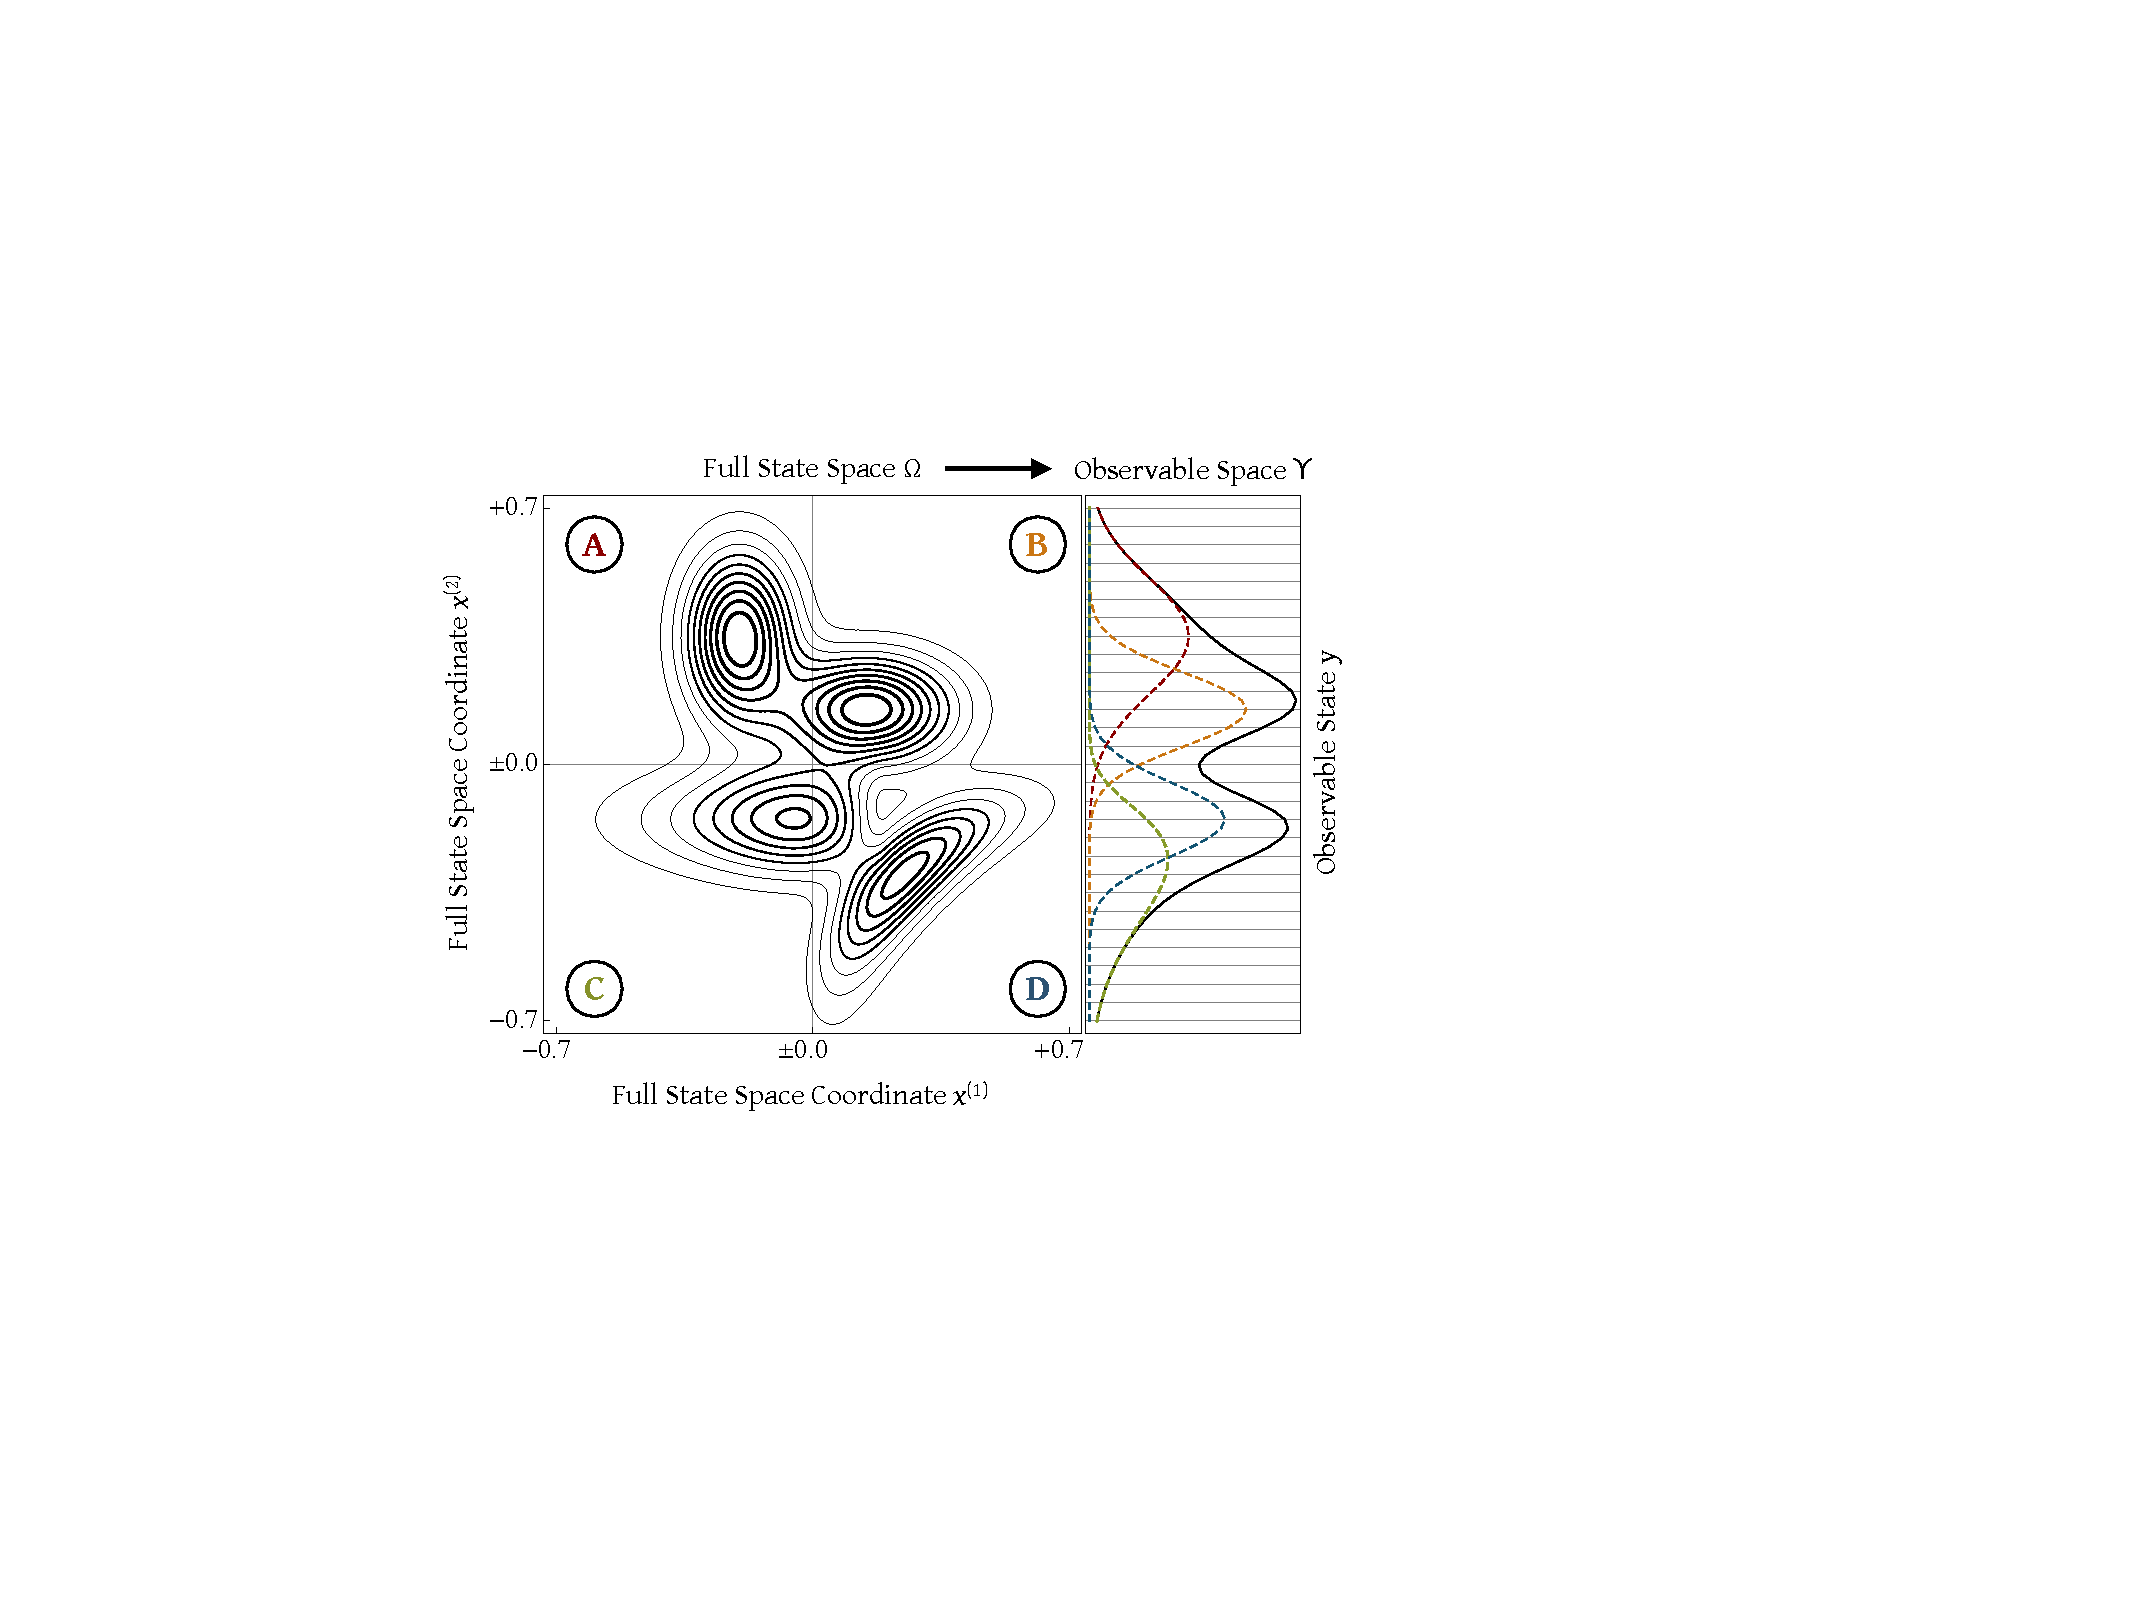
\includegraphics[width=1\columnwidth]{figures/EnergyLandscape}

\label{fig:Energy-Landscape}\textbf{Stationary probability.} Energy
Landscape of illustrative 2D potential\textbf{ }with 4 distinct basins
(metastable states) $A$, $B$, $C$ and $D$. The dynamics in full
space $x_{t}\in\Omega$ is mapped onto coordinate $x^{(2)}$ and discretized
into 28 bins constituting the observable space $y_{t}\in\Upsilon$ 
\end{figure}
\begin{figure}
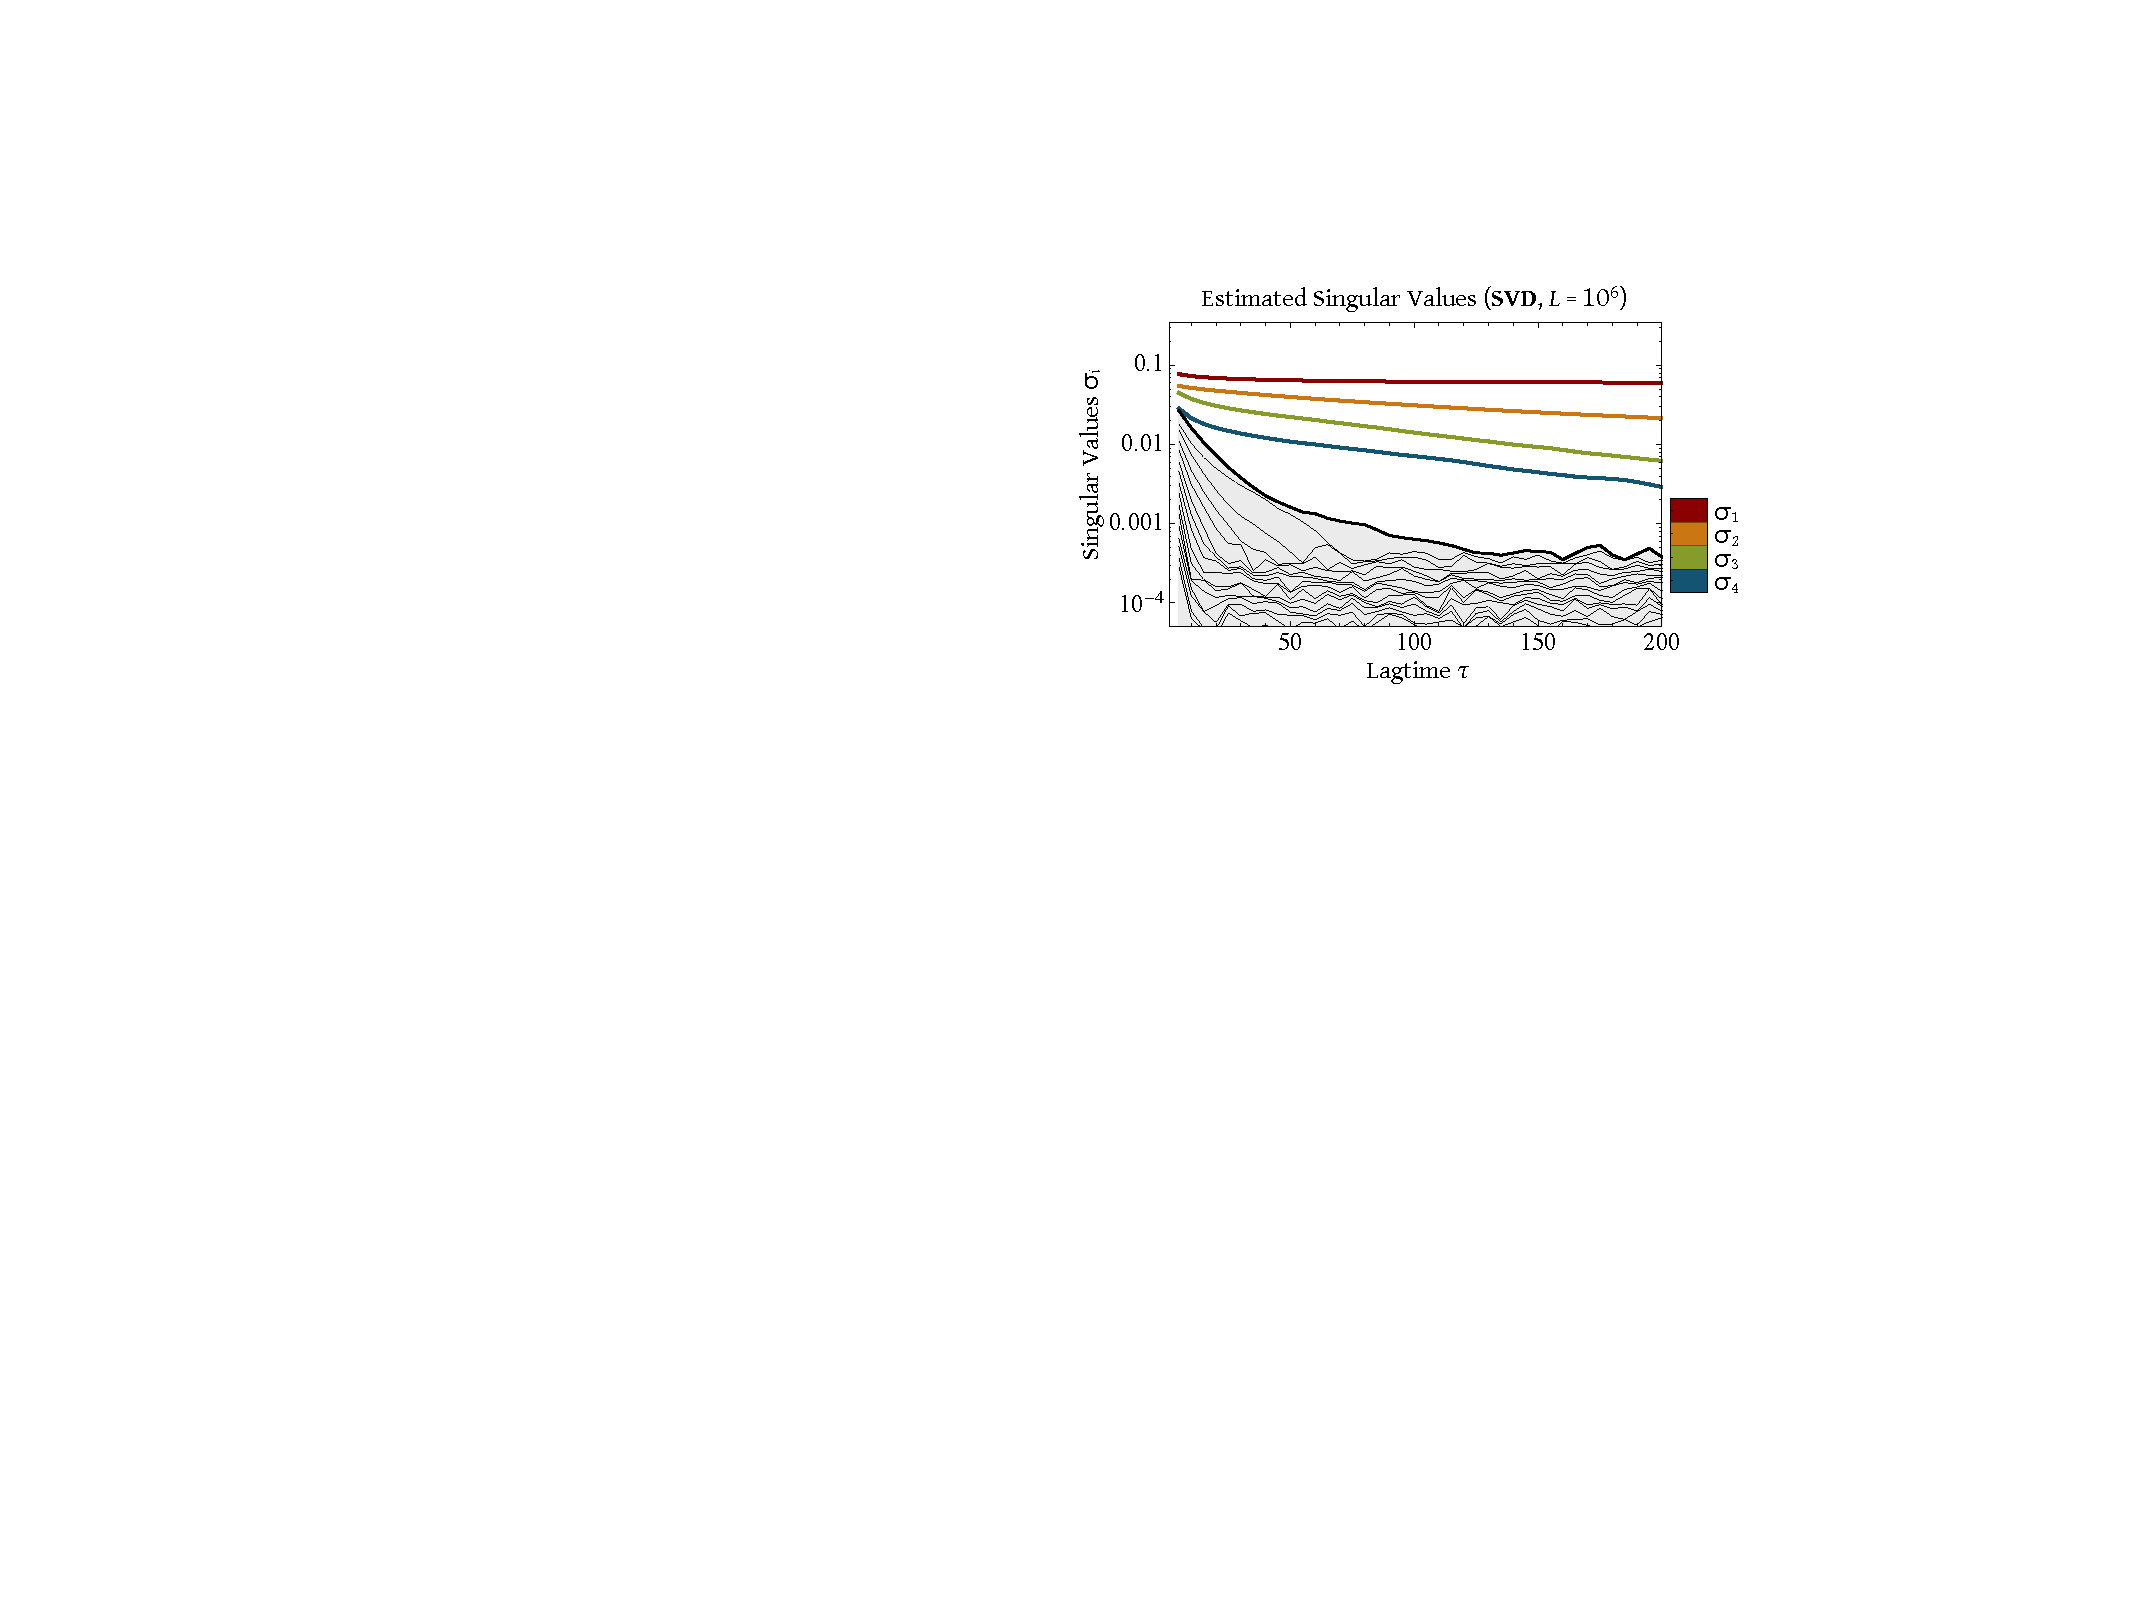
\includegraphics[width=1\columnwidth]{figures/new_SVD}

\label{fig:Singular-values}\textbf{Estimated Singular values. }Singular
values of the correlation matrices $C(\tau)$ symmetrically estimated
from a trajectory ($L=10^{6}$) in the 2D illustrative potential.
Even for small lag times $\tau$ four disctint singular values are
present. For lagtimes $\tau\gtrapprox150$ all but the 4 dominant
singular values have reached noise level and remain approximately
constant.
\end{figure}


\begin{figure}
\begin{centering}
\includegraphics[width=0.9\columnwidth]{\string"figures/Estimated Timescales\string".pdf}
\par\end{centering}

\centering{}\textbf{\label{fig:Estimation-results}Estimated timescales }Various
estimation results for a simple diffusion process in a potential defined
by the stationary distribution in Fig.~\ref{fig:Energy-Landscape}.
Comparison of timescales estimation for $t_{2}$ (yellow), $t_{3}$
(green) and $t_{4}$ (blue) in 3 cases: (thin solid and constant)
exact solution from 28x28 bin discretization of full space, (thick,
solid) \emph{spectral estimate} (SE) for infinite statistics and using
$\tau_{2}=2\tau_{1}$, (dashed) SE estimate for finite statistics
($L=10^{6}$) using $\tau_{2}=2\tau_{1}$ and (dashed) MSM estimate
using single $\tau$. The corresponding arrows in the middle plot
indicate locations of the the used lagtimes $\tau_{1},\tau_{2}$.
The SE estimates converge much faster ($\tau\approx200$) compared
to the MSM method.
\end{figure}


\begin{figure}
\begin{centering}
\includegraphics[width=0.9\columnwidth]{\string"figures/Estimated Eigenvectors\string".pdf}
\par\end{centering}

\centering{}\textbf{\label{fig:Estimation-results-EVec}Estimated projected eigenvectors}
$Q$. (\textbf{\emph{a}}\emph{)} SE at $\tau_{1}=125,\,\tau_{2}=175$
using infinite statistics ($L=\infty$), (\textbf{b}) MSM at $\tau=175$
estimate using infinite statistics. The (\textbf{solid}) lines correspond
to the estimation, while the (\textbf{dashed}) lines are the reference
solution. The smaller the colored areas, the better the approximation.
Although both approaches correctly predict the stationary distribution,
the MSM estimate performs worse than the SE estimate. SE can almost
predict the slowest process ($\lambda_{2}$, yellow) correctly while
process 3 (green) and 4 (blue) are less accurate.
\end{figure}


%%%%%%%%%%%%%%%%%%%%%%%%%%%%%%%%%%%%%%%%%%%%%%%%%%%%%%%%%%%%%%%%%%%%%%%%%%%%%%%%%%%%%%%%%%%%%%%%%%%%%
% MULTI-LAGTIME ESTIMATION
%%%%%%%%%%%%%%%%%%%%%%%%%%%%%%%%%%%%%%%%%%%%%%%%%%%%%%%%%%%%%%%%%%%%%%%%%%%%%%%%%%%%%%%%%%%%%%%%%%%%%

\section{Multi-Lagtime Estimation}

To address the issue of statistical uncertainties we rewrite the problem
into an optimization problem. We use the list of time scales used
in the estimation $\mathcal{T}=\{\tau_{1},\tau_{2}\}$ and write

\[
\left\{ Q,\Lambda\right\} =\underset{Q,\Lambda}{\text{argmin}}\sum_{\tau\in\mathcal{T}}\Vert C(\tau)-Q^{\text{T}}\Lambda(\tau)Q\Vert_{\text{F}}
\]
which is equivalent of estimation the parameters of a PMM as described
above. This can be generalized to more than 2 lagtimes by expanding
$\mathcal{T}$. Fig.~\ref{fig:StatisticalUncertainty} shows estimation
results from the multi-$\tau$ estimation for the 2D example from
Fig.~\ref{fig:Energy-Landscape}. For this we simulated 100 trajectories
starting in the center of state $B$ for 6 different trajectory lengths
$L\in\{50k,80k,100k,150k,200k,500k\}$. With increasing length $L$
the distribution becomes more narrow providing a more reliable estimate.
The MSM estimate (lighter colors) show a systematically too small
estimate compared to the spectral estimations (darker colors).

\begin{figure}
\begin{centering}
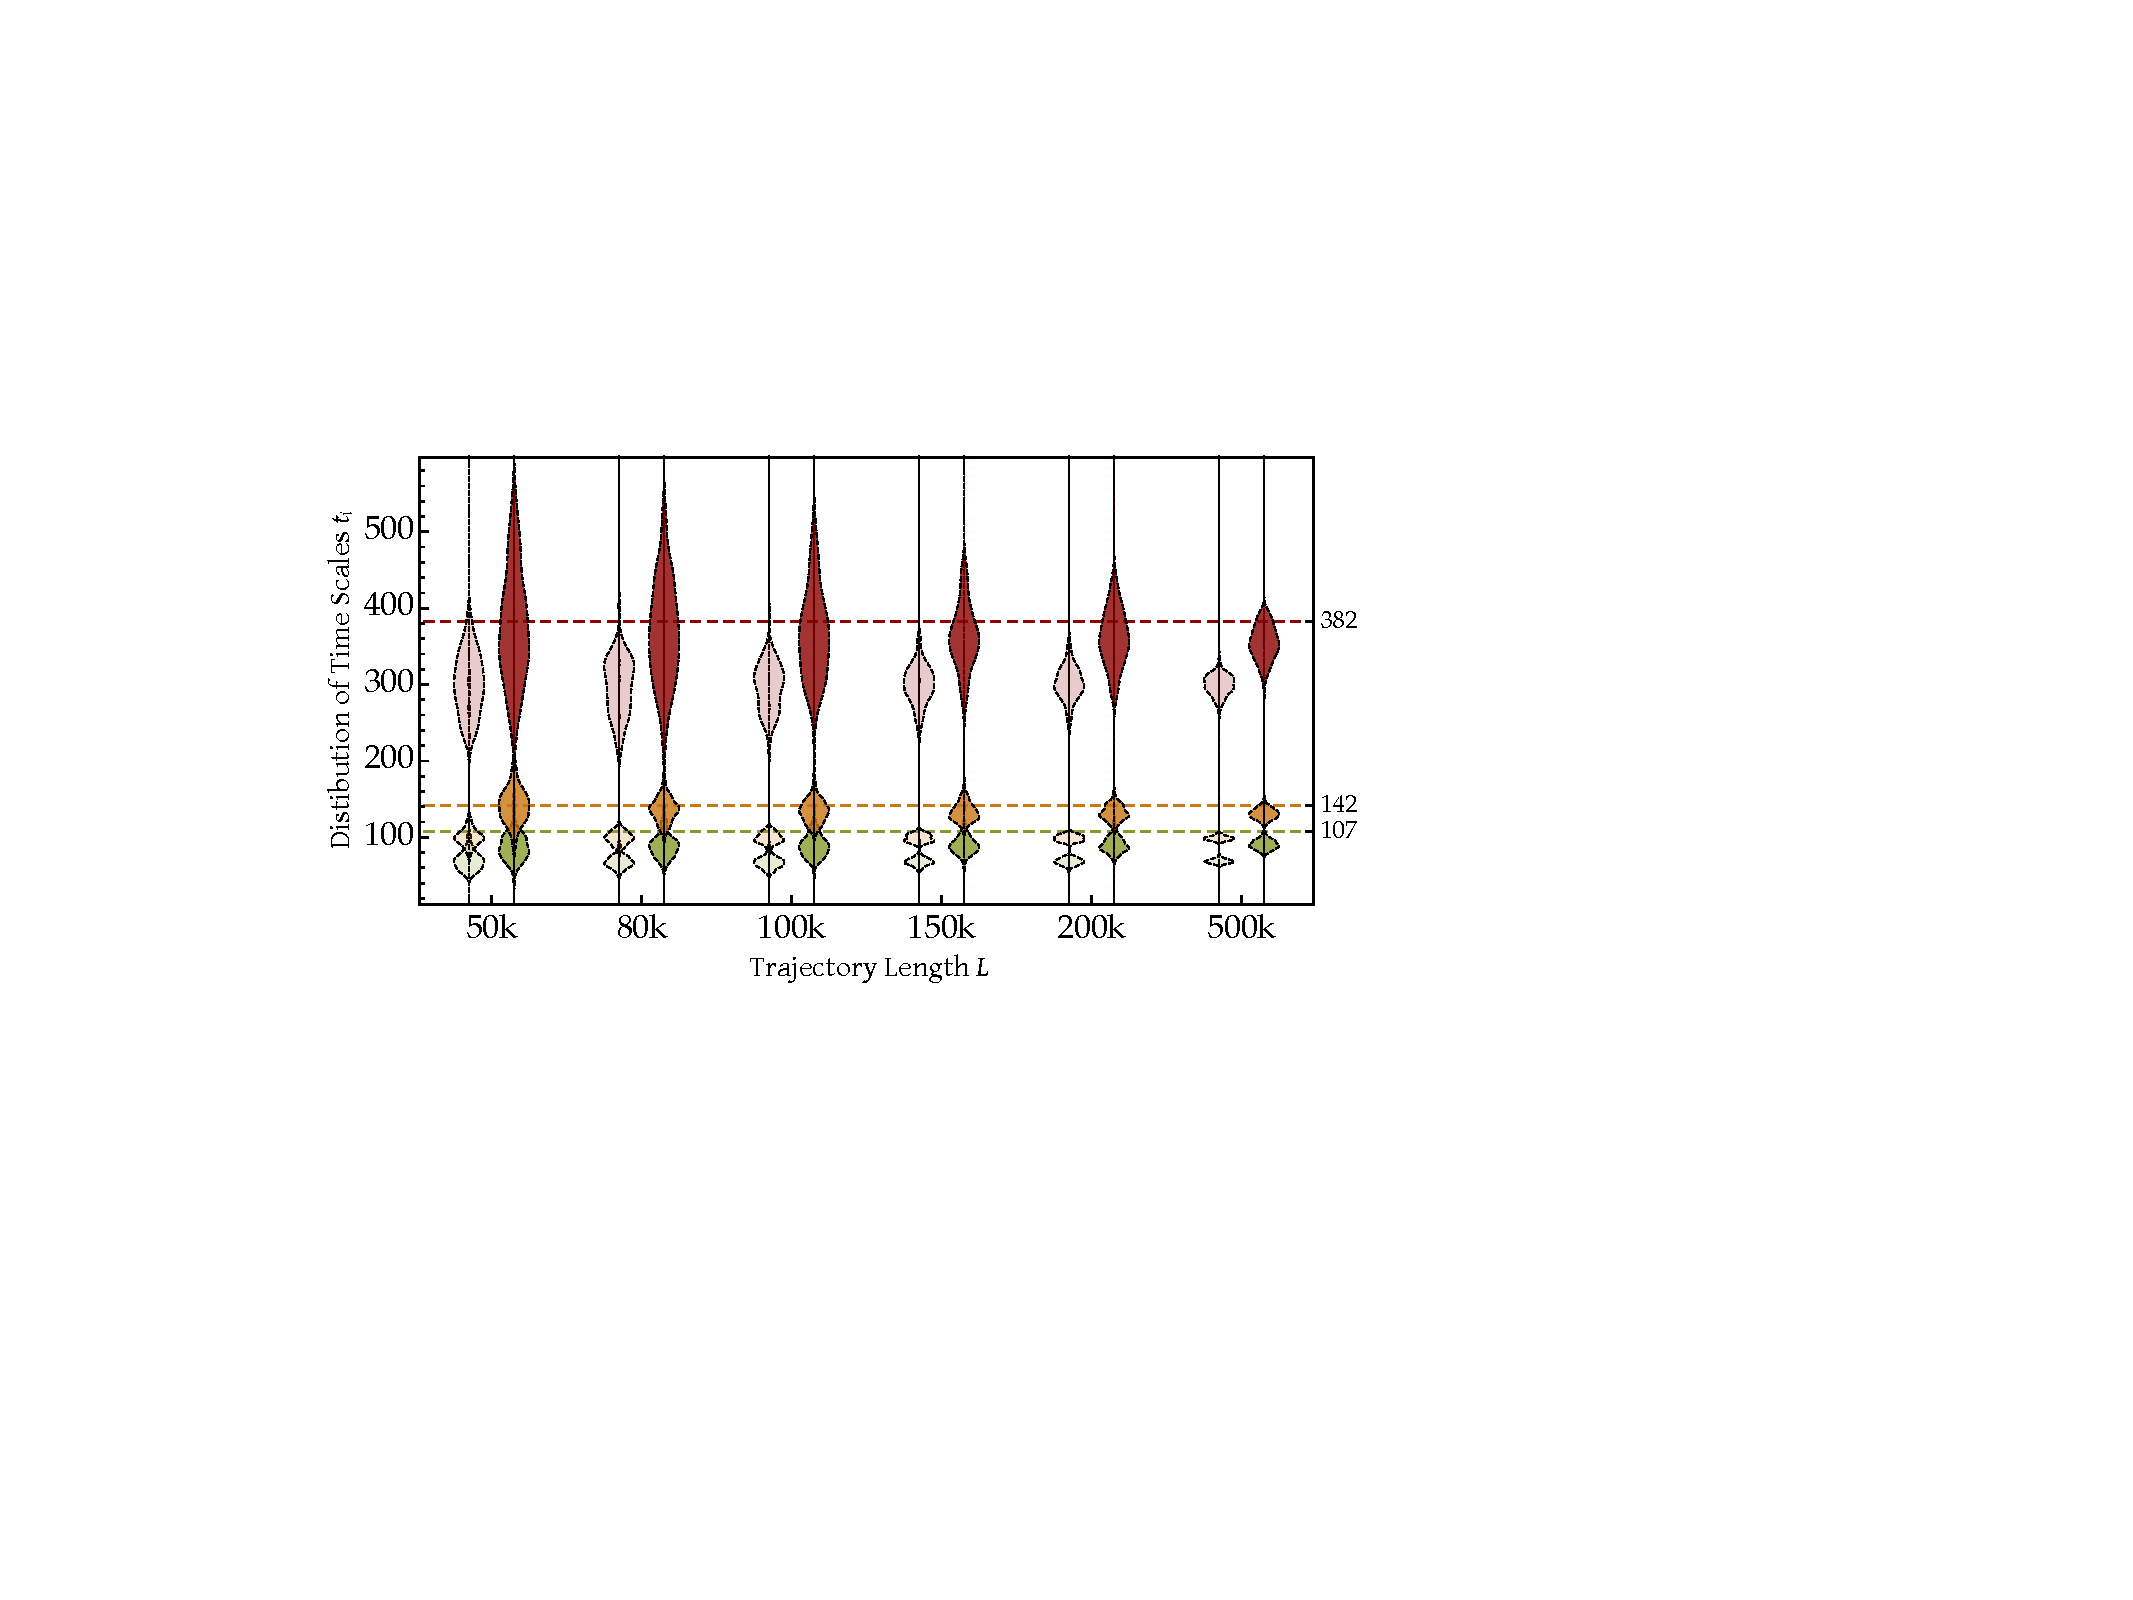
\includegraphics[width=1\columnwidth]{figures/StatisticsEstimation}
\par\end{centering}

\centering{}\label{fig:StatisticalUncertainty}\textbf{Statistical Uncertainty}
Variance in the estimation of timescales due to statistical variation
for a timeseries in the potential of Fig.~\ref{fig:Energy-Landscape}.
All timeseries start in the center of state $B$. Shown are the distributions
of the estimated time scales $t_{i}$ of 100 trajectories for 6 different
trajectory lengths $L\in\{50k,80k,100k,150k,200k,500k\}$. Colors
indicate the processes (red: slowest, yellow: 2nd slowest, green:3rd
slowest). Darker colors refer to the result of Spectral Estimation
with $\mathcal{T}=\{50,\ldots,150\}$ and lighter color is the MSM
estimation of a model computed for $\tau=150$. With incresing trajectory
length the estimation becomes more accurate. While the MSM estimation
is sharper the estimation is significantly less accurate. Both methods
seem to converge to underestimated timescales, as the theory predicts.
\end{figure}

%%%%%%%%%%%%%%%%%%%%%%%%%%%%%%%%%%%%%%%%%%%%%%%%%%%%%%%%%%%%%%%%%%%%%%%%%%%%%%%%%%%%%%%%%%%%%%%%%%%%%
% APO-MYOGLOBIN}
%%%%%%%%%%%%%%%%%%%%%%%%%%%%%%%%%%%%%%%%%%%%%%%%%%%%%%%%%%%%%%%%%%%%%%%%%%%%%%%%%%%%%%%%%%%%%%%%%%%%%

\section{Apo-Myoglobin Example}

We demonstrate the method on the Apo-Myoglobin. {[}Copy experimental
details from PRX publication or give a reference{]}.

In order to illustrate the performance of spectral estimation on real
data, it is applied to optical tweezer measurements of the extension
fluctuations of a biomolecule examined in a recent optical force spectroscopy
study: the H36Q mutant of sperm whale apo-myoglobin at low pH \cite{Elms:2012jb}.
The apo-myoglobin {[}crystal structure shown in Fig. 3(4){]} hops
between unfolded and molten globule states at the experimental pH.
Experimental force trajectory data were generously provided by the
authors of Refs. \cite{Elms:2012jb}. Experimental details are given
therein, but we briefly summarize aspects of the apparatus and experimental
data collection procedure relevant to our analysis. The instrument
used to collect the data sets was a dual-beam counterpropagating optical
trap \cite{Bustamante:wb}. The molecule of interest was tethered
to polystyrene beads by means of dsDNA handles, with one bead suctioned
onto a pipette and the other held in the optical trap. A piezoactuator
controlled the position of the trap and allowed position resolution
to within 0.5 nm, with the instrument operated in passive (equilibrium)
mode such that the trap was stationary relative to the pipette during
data collection. The force on the bead held in the optical trap was
recorded at 50 kHz, with each recorded force trajectory 60 s in duration
resulting in $3\cdot10^{6}$ data points each. From the set of presentes
fibers we chose to analyze fiber no. 6. {[}check how this is mentioned
in Ref. \cite{Elms:2012jb}{]}

Fig.~\ref{fig:ApoMyoglobin} shows estimation results for $\mathcal{T}=\{150,\ldots,500\}$
and computing the projective SVD also at $\tau=150$. The estimations
show a consistent estimation of two processes {[}maybe we can find
a fourth one for 15-17? Actually I checked and it looks like it, but
haven't finished this yet.{]} For \#IDs 15-17 the blue process seems
to switch to a different one at lower bead extensions. 

\begin{figure}
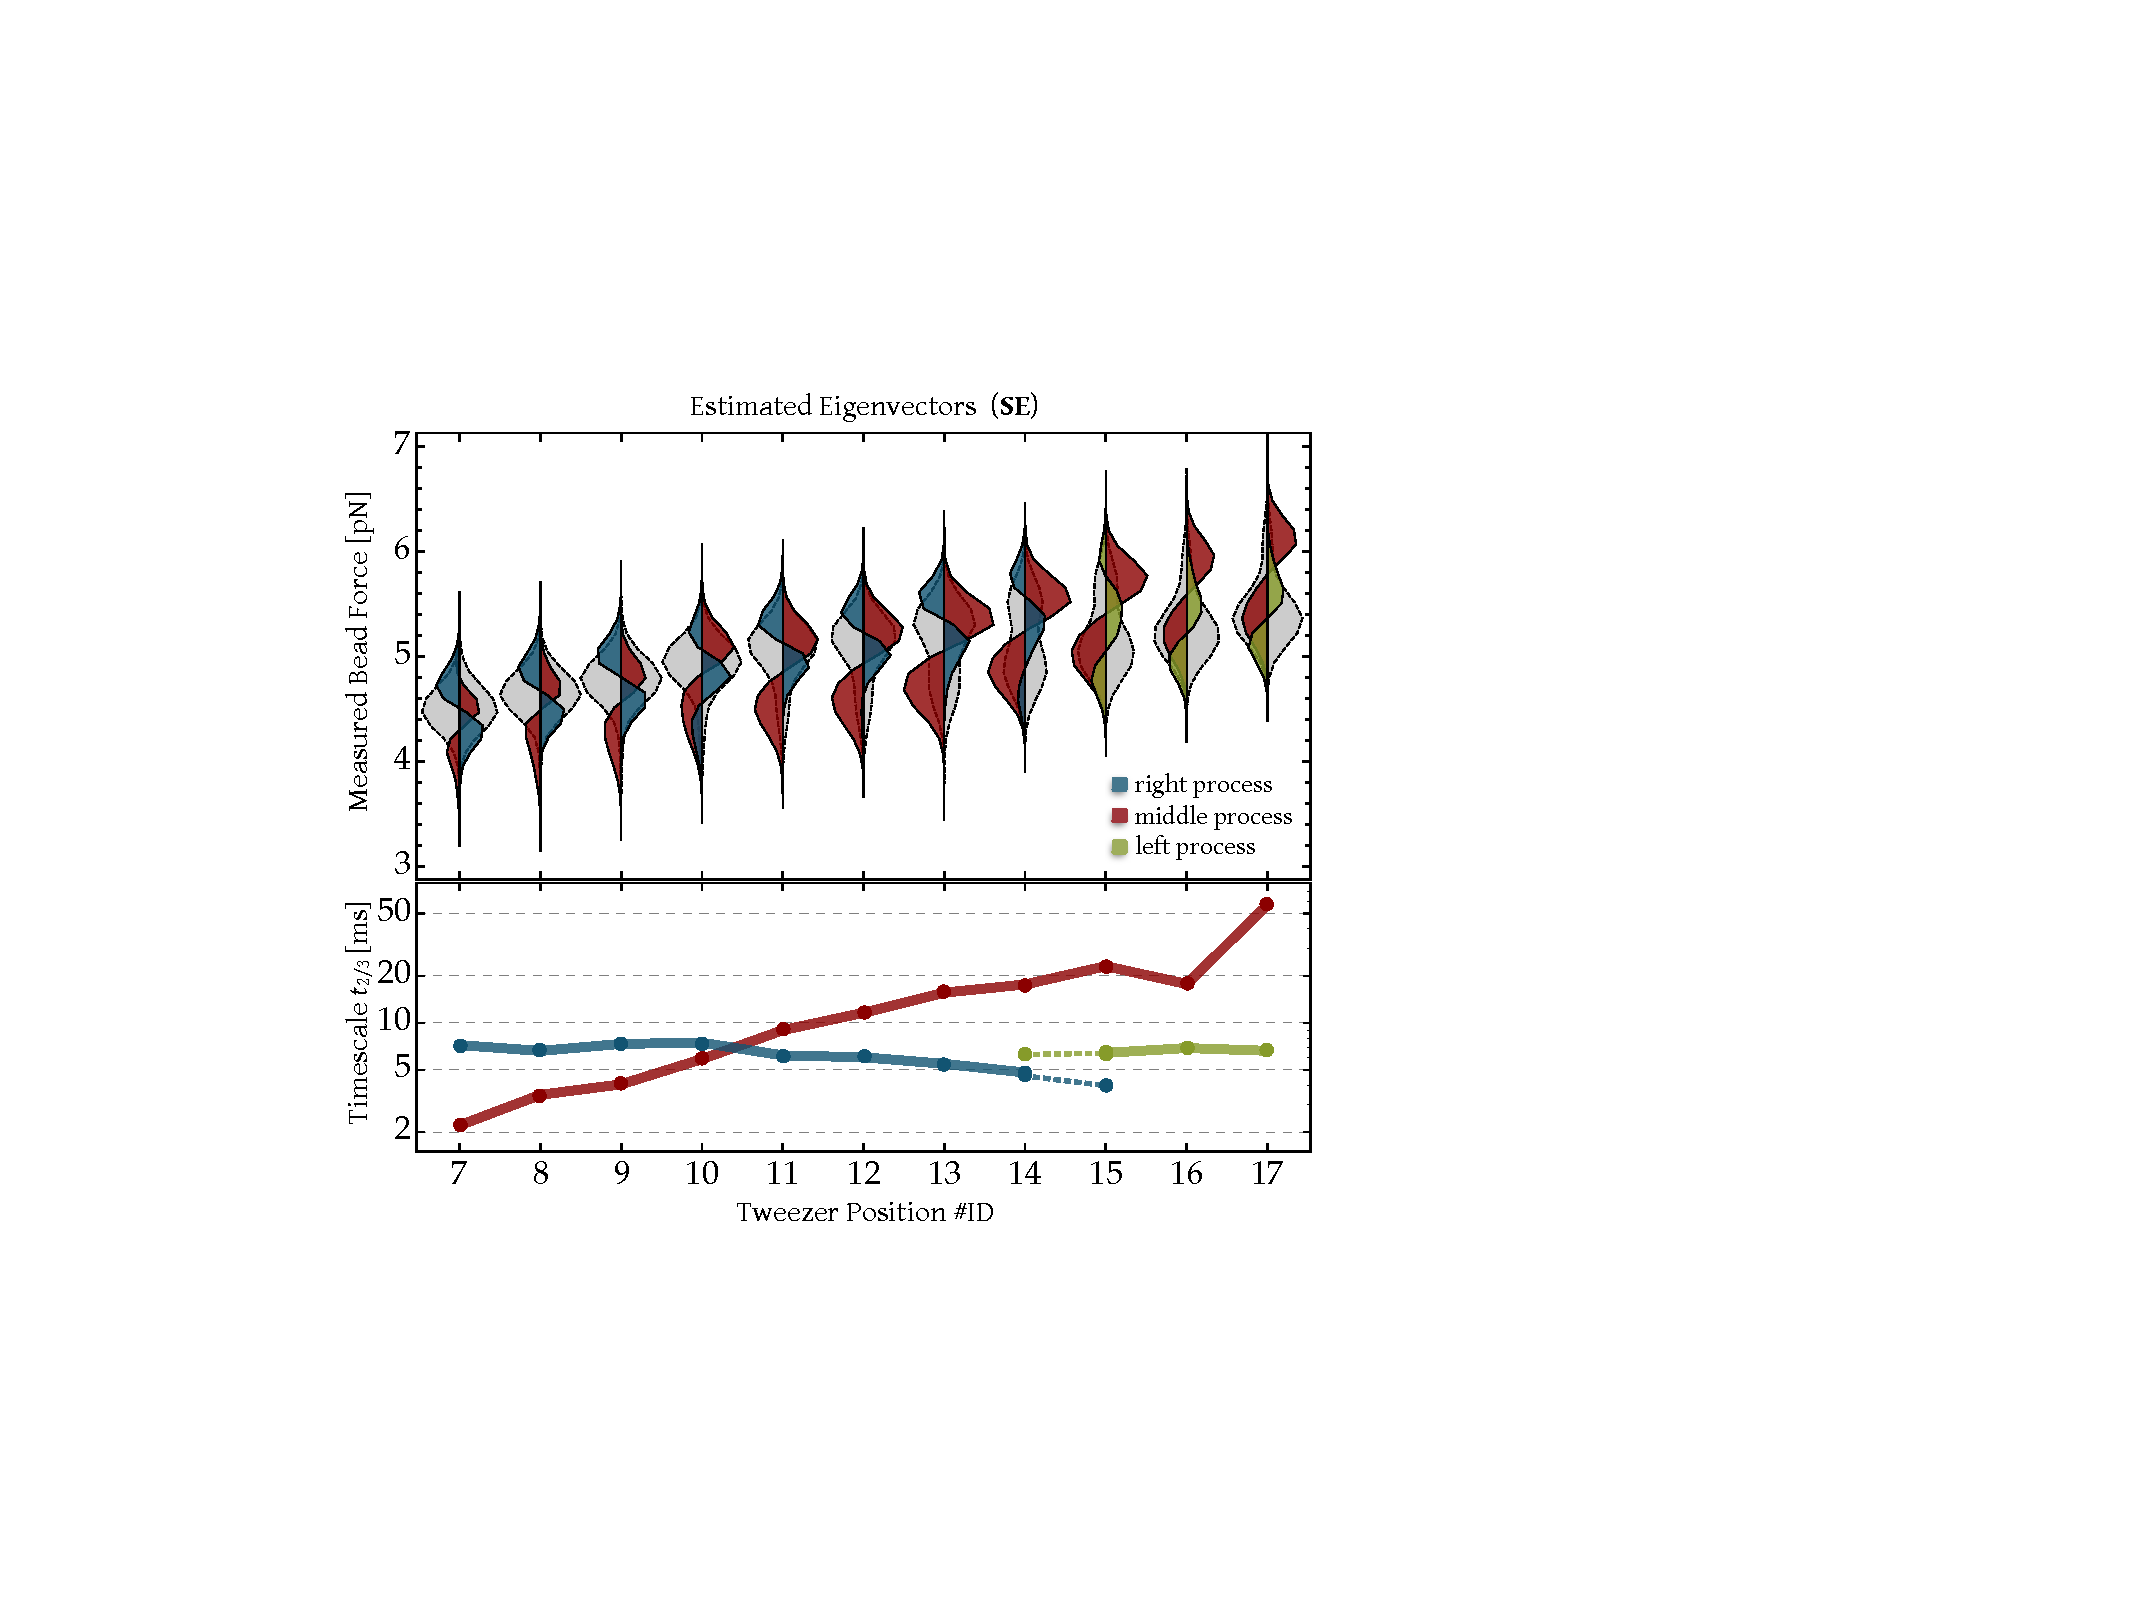
\includegraphics[width=1\columnwidth]{figures/ApoEstimatedTimeScales_V2}

\label{fig:ApoMyoglobin}\textbf{Apo-Myoglobin estimation results}
Results for a series of 11 timeseries recorded in a optical tweezer
experiment of Apo-Myoglobin {[}cite ElmsEtAl, fiber 6{]}. \textbf{(upper)
}3 dominant eigenvectors, which have been assigned according to their
overall shape (\textbf{gray}: stationary distribution, \textbf{red}:
intermediate process, \textbf{blue}: higher force process, \textbf{green}:
lower force process). The shift in measured bead position is due to
an increase in the pulling force, moving the whole protein toward
the force exerting bead. \textbf{(lower) }Time scales for the slowest
processes. Colors are the same as in the upper part. The smaller extended
process shows an almost constant time scale while the other process
gets slower with increasing force {[}check if this is consistent with
prior publication{]}. For positions 14 and 15 also the estimation
with 4 states produced reasonable results which are shown using dashed
lines.
\end{figure}





%%%%%%%%%%%%%%%%%%%%%%%%%%%%%%%%%%%%%%%%%%%%%%%%%%%%%%%%%%%%%%%%%%%%%%%%%%%%%%%%%%%%%%%%%%%%%%%%%%%%%
% CONCLUSION
%%%%%%%%%%%%%%%%%%%%%%%%%%%%%%%%%%%%%%%%%%%%%%%%%%%%%%%%%%%%%%%%%%%%%%%%%%%%%%%%%%%%%%%%%%%%%%%%%%%%%
\section{Conclusion}
\label{section:conclusion}

We presented a novel approach to estimate the parameters $Q$ and
$\Lambda$ of a projected Markov state model (PMM). The method has
been demonstated at a simple illustrative model and shows much improved
convergence in the estimation of the dominant timescales as well as
related projected eigenvectors. Although the sensitivity to statistical
noise has increased the method still provides better results compared
to the MSM approach. The sensitivity can be reduced if the estimation
is reformulated into an optimization problem that fits the result
at more than two lagtimes. We have applied the optimizational approach
to data from Apo-Myoglobin and showed a consistent set of two processes
(maybe four). On first sight the estimation for $m$-PMMs looks identical
to and $m$-state HMM, but it can be shown that HMMs are not able
to capture all possible dynamics of $m$-PMMs and HMMs can model a
subset of the dynamics of PMMs. Thus the HMM solution might be close,
but rarely exact\cite{Noe:2013tx}. Finally, the cases of low-statistics
and non-reversible dynamics is interesting and subject of active research.





%%%%%%%%%%%%%%%%%%%%%%%%%%%%%%%%%%%%%%%%%%%%%%%%%%%%%%%%%%%%%%%%%%%%%%%%%%%%%%%%%%%%%%%%%%%%%%%%%%%%%
% ACKNOWLEDGMENTS
%%%%%%%%%%%%%%%%%%%%%%%%%%%%%%%%%%%%%%%%%%%%%%%%%%%%%%%%%%%%%%%%%%%%%%%%%%%%%%%%%%%%%%%%%%%%%%%%%%%%%
\section{Acknowledgments}
\label{section:acknowledgments}

The authors would like to thank Ralf Banisch for stimulating discussions
on the topic. JHP acknowledges support from the DFG research center
\textsc{Matheon}. HW {[}missing{]} . FN acknowledges funding from
DFG grant NO 825/2-2 and ERC starting grant 'pcCell' \textquotedbl{}.
JDC acknowledges funding from {[}@JDC: missing{]}


%%%%%%%%%%%%%%%%%%%%%%%%%%%%%%%%%%%%%%%%%%%%%%%%%%%%%%%%%%%%%%%%%%%%%%%%%%%%%%%%%%%%%%%%%%%%%%%%%%%%%%
% BIBLIOGRAPHY
%%%%%%%%%%%%%%%%%%%%%%%%%%%%%%%%%%%%%%%%%%%%%%%%%%%%%%%%%%%%%%%%%%%%%%%%%%%%%%%%%%%%%%%%%%%%%%%%%%%%%%

%\bibliographystyle{prsty} 
\bibliography{bib/complete.bib}

\end{document}